\documentclass[a4paper,10pt]{article}
\usepackage[T1]{fontenc}
\usepackage[utf8]{inputenc}
\usepackage[english]{babel}
\usepackage{lmodern}
\usepackage[top=1.6cm,bottom=1.8cm,left=1.9cm,right=1.9cm]{geometry}
\usepackage{titlesec,enumitem,xcolor,graphicx,lastpage,fancyhdr}
\usepackage{fontawesome5}
\usepackage[hidelinks]{hyperref}

\hypersetup{colorlinks=true,urlcolor=blue!70!black,linkcolor=blue!70!black}
\pagestyle{fancy}\fancyhf{}\renewcommand{\headrulewidth}{0pt}
\fancyfoot[C]{\small\color{gray}Page \thepage\ of \pageref{LastPage}}
\setlength{\parindent}{0pt}

\titleformat{\section}{\large\bfseries\color{blue!70!black}}{}{0em}{}[\vspace{-0.7em}\rule{\textwidth}{0.5pt}]
\titlespacing{\section}{0pt}{9pt}{5pt}
\setlist[itemize]{leftmargin=1.1em,itemsep=2pt,topsep=2pt,parsep=0pt}
\newcommand{\role}[4]{\vspace{3pt}\noindent\hspace{0.6em}\parbox[t]{0.38\textwidth}{\raggedright\textbf{#1}}\hfill\parbox[t]{0.58\textwidth}{\raggedleft\textit{#2}}\\{\textit{#3}\hfill\textit{#4}}\vspace{1pt}}

\begin{document}
\noindent
\begin{minipage}[t]{0.78\textwidth}
\vspace{0pt}
{\huge\bfseries Prabhavit Gupta}\\[8pt]
{\small \faPhone\ +39-351-610-7807 \quad \faEnvelope\ \href{mailto:prabhavitg@gmail.com}{prabhavitg@gmail.com} \quad \faLinkedin\ \href{https://www.linkedin.com/in/prabhavit/}{Linkedin} \quad \faMapMarker*\ Venice, Italy}
\end{minipage}\hfill
\begin{minipage}[t]{0.18\textwidth}
\vspace{0pt}\raggedleft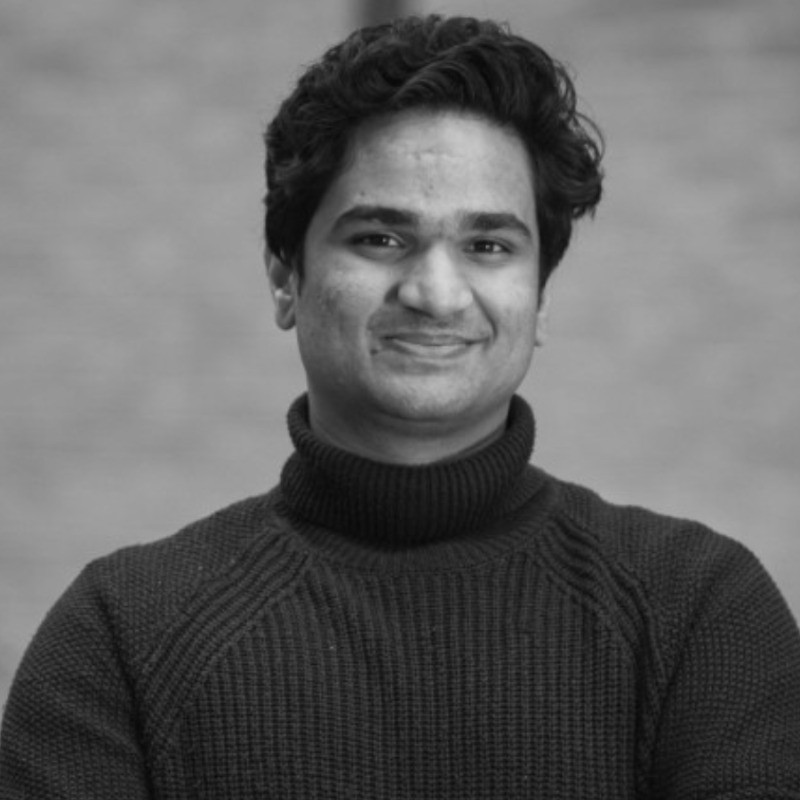
\includegraphics[width=2.3cm,height=2.3cm,keepaspectratio]{photo.jpg}
\end{minipage}

\section{Career Summary}
\begin{itemize}
\item Web and automation developer integrating external APIs, CRM systems, and automated booking workflows.
\item Experience delivering frontend features, Figma implementations, unit testing, and quality assurance across European projects.
\item Oversees FlowSpace's migration from Bubble.io to Next.js and Laravel and documents product logic with developers.
\end{itemize}

\section{Technical Skills}
\begin{itemize}
\item \textbf{AI/ML} -- API integration, AI Agents, RAG, Chatbot development, Eden AI, OpenAI/ChatGPT integration
\item \textbf{Automation} -- n8n, Playwright; CRM integrations, lead capture, data processing and workflow automation
\item \textbf{Development} -- Claude Code, Laravel, Typescript; Next.js migration, Bubble.io, Supabase
\item \textbf{Project/Design} -- Figma, Jira, GitHub, Postman, Trello
\end{itemize}

\section{Visa \& Language}
\begin{itemize}
\item \textbf{Language} -- Hindi (Native), English (Professional), Italian (Beginner)
\item \textbf{Work Authorization} -- European Long Term Residence Permit (Italy).
\end{itemize}

\section{Professional Experience}
\role{\href{https://flowspace.co}{FlowSpace.co}}{Lead Developer (Full time, Freelance)}{London, UK}{Mar 2024 -- Ongoing}
\begin{itemize}
\item \textbf{Product Responsibilities:}
\begin{itemize}[label=--]
\item Scaled the platform from 2,000 to 4,500+ users through iterative product development.
\item Overseeing the migration from Bubble.io to Next.js and Laravel.
\item Collaborated with developers to document product logic and business logic.
\item Facilitated communication between the internal team and the agency.
\item Streamlined customer support with AI agents.
\end{itemize}
\item \textit{Tools: Playwright, Jira, GoogleSheet, Clickup, Miro, Google Analytics, Microsoft Clarity}
\item \textbf{Technical Responsibilities:}
\begin{itemize}[label=--]
\item Built AI tools to process and scrape data for platform listings.
\item Integrated Office Rnd and Nexudus APIs for automated bookings.
\item Consolidated leads in the CRM and automated lead capture through CRM integrations.
\item Built GTM automations for the sales funnel, lead enrichment, and outbound.
\item Built an AI tool to process data and increase listings on the platform.
\item Overseeing the migration from Bubble.io to Next.js and Laravel.
\item Developed a tool for companies to calculate commute times.
\item \textit{Tools: Claude Code, n8n, Bubble.io, Postman, Jira, Github, Laravel, Typescript}
\end{itemize}
\end{itemize}

\role{Urlink}{Project Manager and AI Assisted Developer (Freelance)}{Barcelona, Spain}{April 2025 -- July 2025}
\begin{itemize}
\item Built platform logic using AI-assisted development.
\item Implemented interfaces created with AI.
\item Built automations based on client requirements.
\item \textit{Tools: Github, Netlify, Supabase, bolt.new}
\end{itemize}

\newpage
\role{UltraStrategy.com}{Automation Developer (Collaborator)}{France}{Dec 2024 -- May 2025}
\begin{itemize}
\item Built a CV parsing tool using n8n and Eden AI.
\item Developed a platform for different user profiles.
\item \textit{Tools: n8n, Eden AI, Bubble.io}
\end{itemize}

\role{Qomodo}{AI and Low-Code Developer (Collaborator)}{Milan, Italy}{2024 -- Jan 2025}
\begin{itemize}
\item Implemented Figma designs.
\item Built a dashboard for companies to manage their branches.
\item \textit{Tools: Bubble}
\end{itemize}

\role{Get2Germany.com}{Lead Developer and Automation Specialist (Part time)}{Berlin, Germany}{Jan 2024 -- May 2024}
\begin{itemize}
\item Integrated Google APIs for platform tracking.
\item Implemented Figma designs in Bubble.
\item Built the platform and optimized its database.
\item Developed AI automation tools to find courses, internships, and jobs.
\item \textit{Tools: Bubble.io, Figma, Trello, n8n}
\end{itemize}

\role{Clubee.com}{Low Code Developer and Quality Assurance (Full time, Freelance)}{Foetz, Luxembourg}{Sep 2023 -- Aug 2024}
\begin{itemize}
\item Integrated the Clubee API across the frontend.
\item Performed unit testing and quality assurance for new features.
\item Built tools for domain integration, the shop, and the federation dashboard.
\item \textit{Tools: Bubble.io, Figma, GitHub, Postman}
\end{itemize}

\role{Tractionboard.co}{Low-Code Developer (Internship)}{Utrecht, Netherlands}{Aug 2023 -- Oct 2023}
\begin{itemize}
\item Integrated ChatGPT/OpenAI and Sendgrid.
\item Implemented Figma designs in Bubble.
\item Built responsive interfaces and fixed bugs.
\item Implemented Google Ads 4.
\item \textit{Tools: Bubble.io, Figma, Sendgrid, ChatGPT}
\end{itemize}

\section{Education}
\role{Ca' Foscari University of Venice}{Bachelor's in Philosophy, International Studies \& Economics with Minor in Entrepreneurship}{Venice, Italy}{Oct 2020 -- Jun 2024}

\section{Certifications}
\begin{itemize}
\item Microsoft Copilot Studio Agent Academy
\item Microsoft - Introduction to building AI agents
\item Microsoft Power Automate
\item Tray.AI Build Practitioner -- September 2024
\item Tray.AI Build Foundations
\end{itemize}
\end{document}
